\begin{figure}[p]\centering
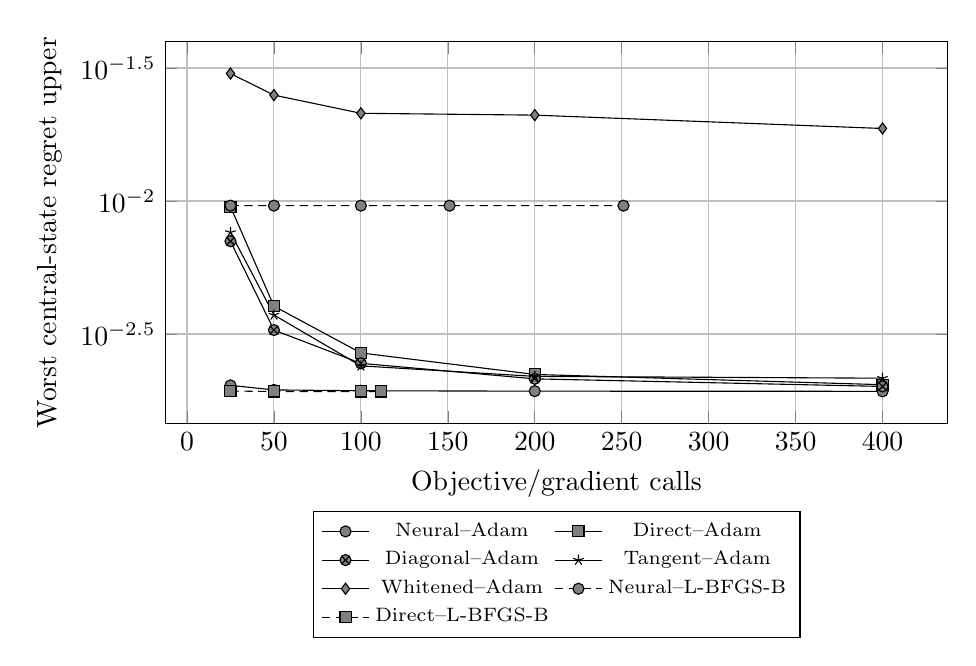
\begin{tikzpicture}\begin{axis}[width=.95\textwidth,height=.53\textwidth,ymode=log,xlabel={Objective/gradient calls},ylabel={Worst central-state regret upper},legend style={font=\scriptsize,at={(0.5,-0.23)},anchor=north,legend columns=2},cycle list name=black white,grid=major]
\addplot+ coordinates {(25,0.00202746061517) (50,0.00194950145597) (100,0.0019349101657) (200,0.00192863167763) (400,0.00192571291215)};\addlegendentry{Neural--Adam}
\addplot+ coordinates {(25,0.0095266270982) (50,0.00402455251775) (100,0.00268452213393) (200,0.00222821354893) (400,0.00203922705228)};\addlegendentry{Direct--Adam}
\addplot+ coordinates {(25,0.00706010753057) (50,0.00327282233924) (100,0.00245383492174) (200,0.00214493939263) (400,0.00200873460523)};\addlegendentry{Diagonal--Adam}
\addplot+ coordinates {(25,0.00761882459032) (50,0.00372955082102) (100,0.00239992613935) (200,0.00219163615955) (400,0.00215723161614)};\addlegendentry{Tangent--Adam}
\addplot+ coordinates {(25,0.0301532988188) (50,0.025022949821) (100,0.0213764994292) (200,0.0210368831176) (400,0.0187420285412)};\addlegendentry{Whitened--Adam}
\addplot+ coordinates {(25,0.00960967109684) (50,0.00960832614177) (100,0.00960832614177) (151,0.00960832614177) (251,0.00960832614177)};\addlegendentry{Neural--L-BFGS-B}
\addplot+ coordinates {(25,0.00193054208314) (50,0.00192368858146) (100,0.00192344285797) (111.5,0.00192344285797) (111.5,0.00192344285797)};\addlegendentry{Direct--L-BFGS-B}
\end{axis}\end{tikzpicture}
\caption{All five prospective checkpoints, rule 8/16. Ordinate: worse regret bound across two seeds; abscissa: mean actual calls or cost. Lines connect recorded checkpoints, not extra observations. Certification is serial replay, so cumulative cost is reconstructed rather than directly timed online wall time.}\end{figure}
\begin{figure}[p]\centering
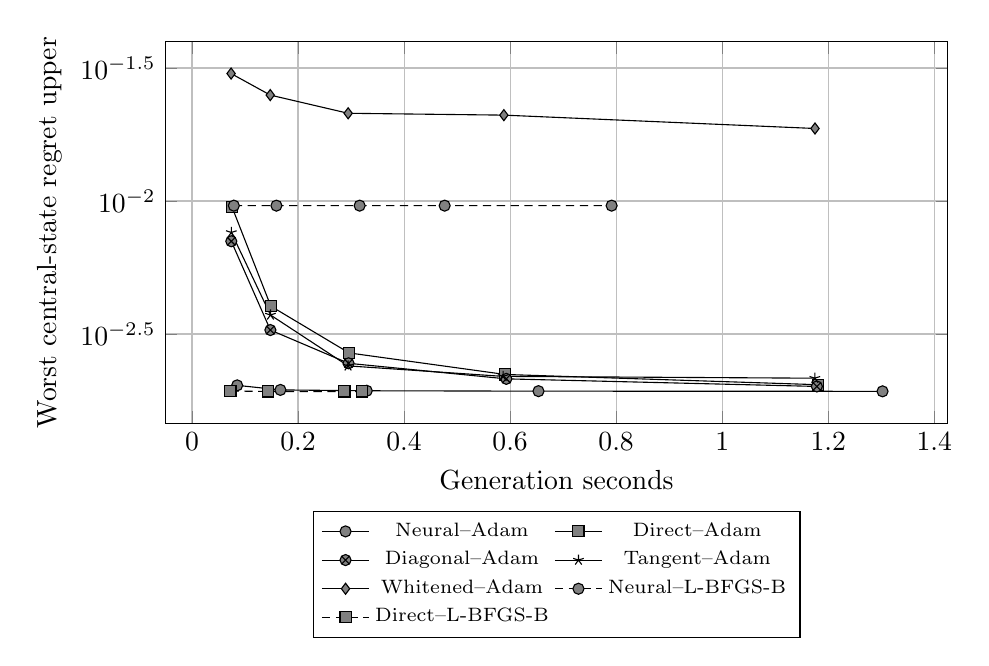
\begin{tikzpicture}\begin{axis}[width=.95\textwidth,height=.53\textwidth,ymode=log,xlabel={Generation seconds},ylabel={Worst central-state regret upper},legend style={font=\scriptsize,at={(0.5,-0.23)},anchor=north,legend columns=2},cycle list name=black white,grid=major]
\addplot+ coordinates {(0.085190371,0.00202746061517) (0.1667503465,0.00194950145597) (0.3295984665,0.0019349101657) (0.653513655,0.00192863167763) (1.302440713,0.00192571291215)};\addlegendentry{Neural--Adam}
\addplot+ coordinates {(0.075180235,0.0095266270982) (0.1486825755,0.00402455251775) (0.296327056,0.00268452213393) (0.5904344295,0.00222821354893) (1.180453165,0.00203922705228)};\addlegendentry{Direct--Adam}
\addplot+ coordinates {(0.0740899265,0.00706010753057) (0.1478579445,0.00327282233924) (0.29530931,0.00245383492174) (0.592865943,0.00214493939263) (1.178593873,0.00200873460523)};\addlegendentry{Diagonal--Adam}
\addplot+ coordinates {(0.074168682,0.00761882459032) (0.1480145975,0.00372955082102) (0.294343687,0.00239992613935) (0.5867250355,0.00219163615955) (1.174718289,0.00215723161614)};\addlegendentry{Tangent--Adam}
\addplot+ coordinates {(0.0737032085,0.0301532988188) (0.1476078865,0.025022949821) (0.294509208,0.0213764994292) (0.5882263245,0.0210368831176) (1.1750650195,0.0187420285412)};\addlegendentry{Whitened--Adam}
\addplot+ coordinates {(0.0789034485,0.00960967109684) (0.1592275735,0.00960832614177) (0.3161687915,0.00960832614177) (0.476508957,0.00960832614177) (0.791457727,0.00960832614177)};\addlegendentry{Neural--L-BFGS-B}
\addplot+ coordinates {(0.0725573095,0.00193054208314) (0.143977069,0.00192368858146) (0.287535419,0.00192344285797) (0.320645736,0.00192344285797) (0.320645736,0.00192344285797)};\addlegendentry{Direct--L-BFGS-B}
\end{axis}\end{tikzpicture}
\caption{All five prospective checkpoints, rule 8/16. Ordinate: worse regret bound across two seeds; abscissa: mean actual calls or cost. Lines connect recorded checkpoints, not extra observations. Certification is serial replay, so cumulative cost is reconstructed rather than directly timed online wall time.}\end{figure}
\begin{figure}[p]\centering
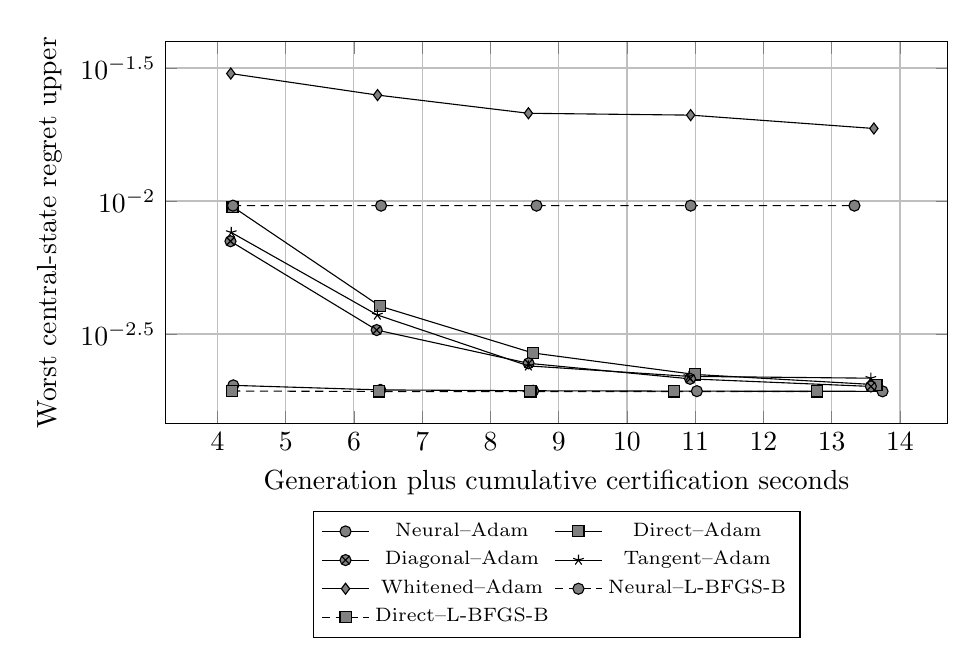
\begin{tikzpicture}\begin{axis}[width=.95\textwidth,height=.53\textwidth,ymode=log,xlabel={Generation plus cumulative certification seconds},ylabel={Worst central-state regret upper},legend style={font=\scriptsize,at={(0.5,-0.23)},anchor=north,legend columns=2},cycle list name=black white,grid=major]
\addplot+ coordinates {(4.2325075875,0.00202746061517) (6.38725457,0.00194950145597) (8.6262041475,0.0019349101657) (11.024284957,0.00192863167763) (13.744141597,0.00192571291215)};\addlegendentry{Neural--Adam}
\addplot+ coordinates {(4.2206801585,0.0095266270982) (6.381376692,0.00402455251775) (8.619138067,0.00268452213393) (10.996279922,0.00222821354893) (13.6556989775,0.00203922705228)};\addlegendentry{Direct--Adam}
\addplot+ coordinates {(4.191122324,0.00706010753057) (6.3333627775,0.00327282233924) (8.558650344,0.00245383492174) (10.9247086365,0.00214493939263) (13.573812392,0.00200873460523)};\addlegendentry{Diagonal--Adam}
\addplot+ coordinates {(4.2025912425,0.00761882459032) (6.342875523,0.00372955082102) (8.555609914,0.00239992613935) (10.906881014,0.00219163615955) (13.573027871,0.00215723161614)};\addlegendentry{Tangent--Adam}
\addplot+ coordinates {(4.1954870185,0.0301532988188) (6.34602037,0.025022949821) (8.5564573105,0.0213764994292) (10.9332736165,0.0210368831176) (13.617223264,0.0187420285412)};\addlegendentry{Whitened--Adam}
\addplot+ coordinates {(4.2272505005,0.00960967109684) (6.397464538,0.00960832614177) (8.6747814735,0.00960832614177) (10.933882636,0.00960832614177) (13.33243796,0.00960832614177)};\addlegendentry{Neural--L-BFGS-B}
\addplot+ coordinates {(4.21547588,0.00193054208314) (6.3650718485,0.00192368858146) (8.585956683,0.00192344285797) (10.6934989265,0.00192344285797) (12.7836852795,0.00192344285797)};\addlegendentry{Direct--L-BFGS-B}
\end{axis}\end{tikzpicture}
\caption{All five prospective checkpoints, rule 8/16. Ordinate: worse regret bound across two seeds; abscissa: mean actual calls or cost. Lines connect recorded checkpoints, not extra observations. Certification is serial replay, so cumulative cost is reconstructed rather than directly timed online wall time.}\end{figure}
\begin{figure}[p]\centering
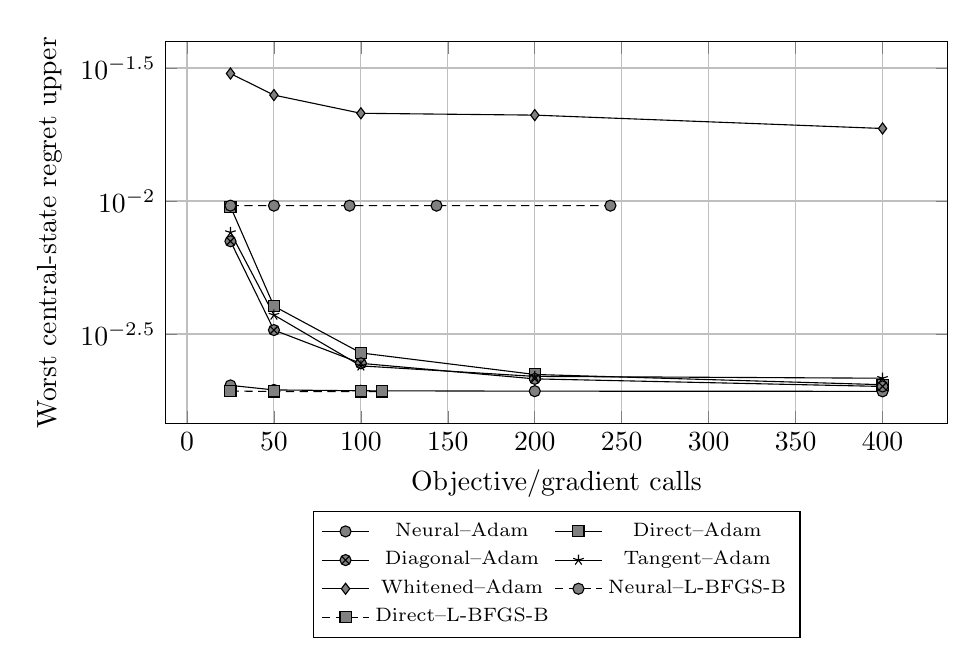
\begin{tikzpicture}\begin{axis}[width=.95\textwidth,height=.53\textwidth,ymode=log,xlabel={Objective/gradient calls},ylabel={Worst central-state regret upper},legend style={font=\scriptsize,at={(0.5,-0.23)},anchor=north,legend columns=2},cycle list name=black white,grid=major]
\addplot+ coordinates {(25,0.00202723548536) (50,0.00194949735872) (100,0.00193488823121) (200,0.00192861229754) (400,0.00192570475209)};\addlegendentry{Neural--Adam}
\addplot+ coordinates {(25,0.00952662525676) (50,0.00402452791078) (100,0.00268447423418) (200,0.00222815961052) (400,0.0020391880294)};\addlegendentry{Direct--Adam}
\addplot+ coordinates {(25,0.00706010725647) (50,0.00327279834644) (100,0.00245378270683) (200,0.00214488965772) (400,0.00200870060725)};\addlegendentry{Diagonal--Adam}
\addplot+ coordinates {(25,0.00761875768147) (50,0.00372953127525) (100,0.00239987631014) (200,0.00219158480394) (400,0.00215718190969)};\addlegendentry{Tangent--Adam}
\addplot+ coordinates {(25,0.0301533002236) (50,0.0250231010271) (100,0.0213767695895) (200,0.0210372187856) (400,0.0187422670181)};\addlegendentry{Whitened--Adam}
\addplot+ coordinates {(25,0.00960965762784) (50,0.00960818012021) (93.5,0.00960818012021) (143.5,0.00960818012021) (243.5,0.00960818012021)};\addlegendentry{Neural--L-BFGS-B}
\addplot+ coordinates {(25,0.00193053282688) (50,0.00192366681516) (100,0.00192366681516) (112,0.00192366681516) (112,0.00192366681516)};\addlegendentry{Direct--L-BFGS-B}
\end{axis}\end{tikzpicture}
\caption{All five prospective checkpoints, rule 12/24. Ordinate: worse regret bound across two seeds; abscissa: mean actual calls or cost. Lines connect recorded checkpoints, not extra observations. Certification is serial replay, so cumulative cost is reconstructed rather than directly timed online wall time.}\end{figure}
\begin{figure}[p]\centering
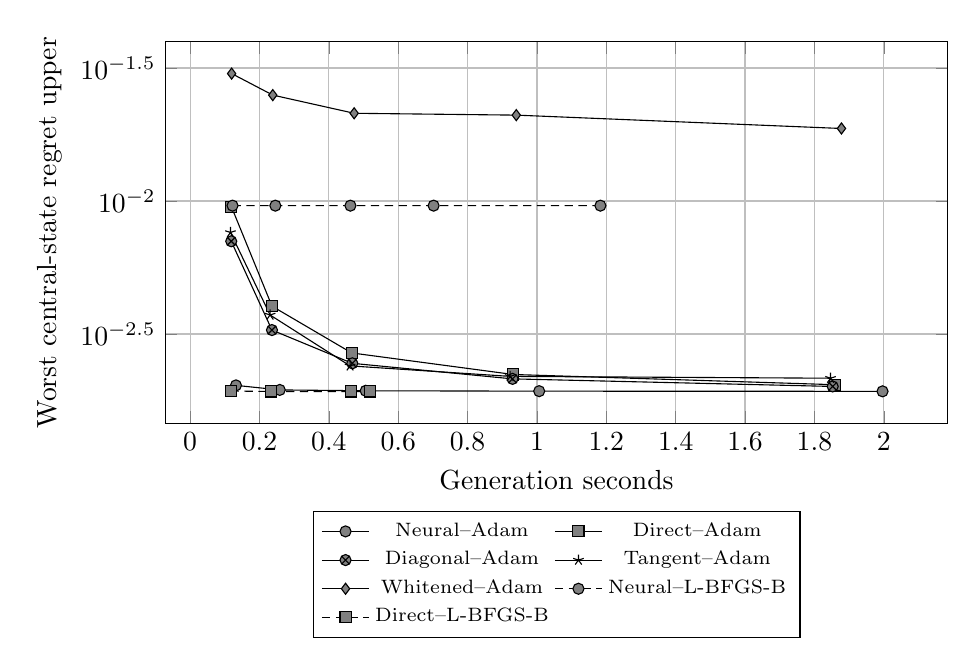
\begin{tikzpicture}\begin{axis}[width=.95\textwidth,height=.53\textwidth,ymode=log,xlabel={Generation seconds},ylabel={Worst central-state regret upper},legend style={font=\scriptsize,at={(0.5,-0.23)},anchor=north,legend columns=2},cycle list name=black white,grid=major]
\addplot+ coordinates {(0.132140211,0.00202723548536) (0.2584085655,0.00194949735872) (0.5062139445,0.00193488823121) (1.0064700815,0.00192861229754) (1.996421088,0.00192570475209)};\addlegendentry{Neural--Adam}
\addplot+ coordinates {(0.118965893,0.00952662525676) (0.236075299,0.00402452791078) (0.4659269885,0.00268447423418) (0.930847039,0.00222815961052) (1.8593667705,0.0020391880294)};\addlegendentry{Direct--Adam}
\addplot+ coordinates {(0.118510522,0.00706010725647) (0.235960516,0.00327279834644) (0.467579756,0.00245378270683) (0.9295740365,0.00214488965772) (1.8527011025,0.00200870060725)};\addlegendentry{Diagonal--Adam}
\addplot+ coordinates {(0.1163361705,0.00761875768147) (0.2305515475,0.00372953127525) (0.461180043,0.00239987631014) (0.9228222955,0.00219158480394) (1.8465210605,0.00215718190969)};\addlegendentry{Tangent--Adam}
\addplot+ coordinates {(0.1196576055,0.0301533002236) (0.238325145,0.0250231010271) (0.4730117845,0.0213767695895) (0.940394887,0.0210372187856) (1.878009586,0.0187422670181)};\addlegendentry{Whitened--Adam}
\addplot+ coordinates {(0.122253171,0.00960965762784) (0.2457344405,0.00960818012021) (0.4622194655,0.00960818012021) (0.7020173285,0.00960818012021) (1.182989959,0.00960818012021)};\addlegendentry{Neural--L-BFGS-B}
\addplot+ coordinates {(0.116861372,0.00193053282688) (0.2337607595,0.00192366681516) (0.464467812,0.00192366681516) (0.5194622975,0.00192366681516) (0.5194622975,0.00192366681516)};\addlegendentry{Direct--L-BFGS-B}
\end{axis}\end{tikzpicture}
\caption{All five prospective checkpoints, rule 12/24. Ordinate: worse regret bound across two seeds; abscissa: mean actual calls or cost. Lines connect recorded checkpoints, not extra observations. Certification is serial replay, so cumulative cost is reconstructed rather than directly timed online wall time.}\end{figure}
\begin{figure}[p]\centering
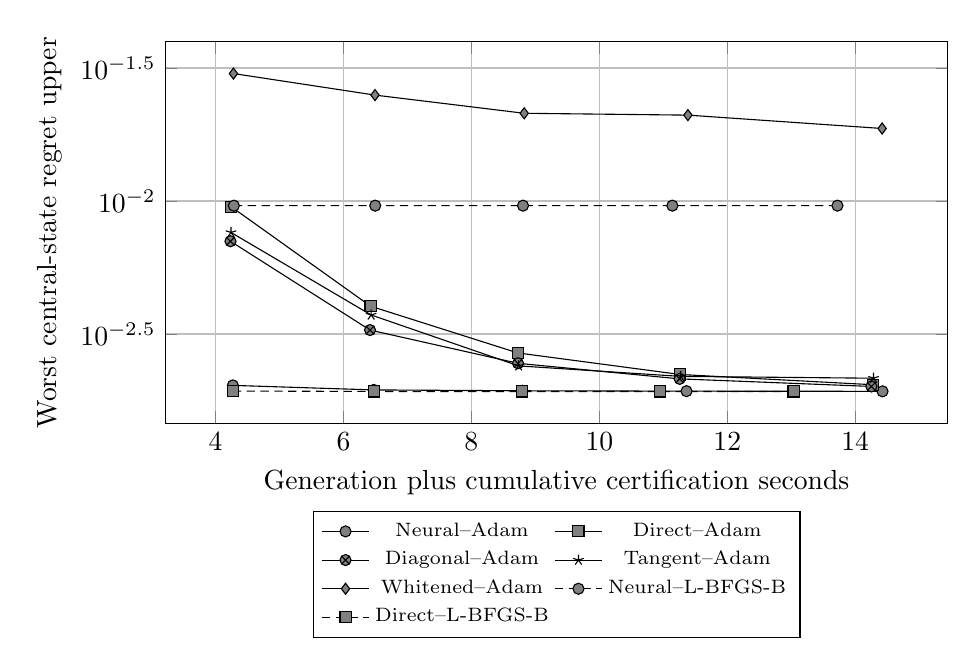
\begin{tikzpicture}\begin{axis}[width=.95\textwidth,height=.53\textwidth,ymode=log,xlabel={Generation plus cumulative certification seconds},ylabel={Worst central-state regret upper},legend style={font=\scriptsize,at={(0.5,-0.23)},anchor=north,legend columns=2},cycle list name=black white,grid=major]
\addplot+ coordinates {(4.2705961555,0.00202723548536) (6.473664638,0.00194949735872) (8.795292758,0.00193488823121) (11.362631499,0.00192861229754) (14.4270221715,0.00192570475209)};\addlegendentry{Neural--Adam}
\addplot+ coordinates {(4.2429324415,0.00952662525676) (6.4232041965,0.00402452791078) (8.7257641485,0.00268447423418) (11.259126115,0.00222815961052) (14.271826742,0.0020391880294)};\addlegendentry{Direct--Adam}
\addplot+ coordinates {(4.233464293,0.00706010725647) (6.4151471165,0.00327279834644) (8.728809561,0.00245378270683) (11.256166668,0.00214488965772) (14.252839068,0.00200870060725)};\addlegendentry{Diagonal--Adam}
\addplot+ coordinates {(4.241808324,0.00761875768147) (6.432651825,0.00372953127525) (8.7384599605,0.00239987631014) (11.2732980455,0.00219158480394) (14.2860555285,0.00215718190969)};\addlegendentry{Tangent--Adam}
\addplot+ coordinates {(4.2798077365,0.0301533002236) (6.4928988485,0.0250231010271) (8.8257559755,0.0213767695895) (11.3847944025,0.0210372187856) (14.420283594,0.0187422670181)};\addlegendentry{Whitened--Adam}
\addplot+ coordinates {(4.2865569025,0.00960965762784) (6.496318939,0.00960818012021) (8.806823538,0.00960818012021) (11.141311786,0.00960818012021) (13.7219659985,0.00960818012021)};\addlegendentry{Neural--L-BFGS-B}
\addplot+ coordinates {(4.269974264,0.00193053282688) (6.481916768,0.00192366681516) (8.794951505,0.00192366681516) (10.946349913,0.00192366681516) (13.036500431,0.00192366681516)};\addlegendentry{Direct--L-BFGS-B}
\end{axis}\end{tikzpicture}
\caption{All five prospective checkpoints, rule 12/24. Ordinate: worse regret bound across two seeds; abscissa: mean actual calls or cost. Lines connect recorded checkpoints, not extra observations. Certification is serial replay, so cumulative cost is reconstructed rather than directly timed online wall time.}\end{figure}

